\section{Functional Damage Explains More Than Raw Magnitude}
\label{sec:damage}

We next discriminate between two simple descriptions of the response. A raw-
magnitude account predicts that interventions moving the local activation by a
similar amount should produce similar top-1 damage. A functional-damage account
instead predicts that the change in output distribution is the more informative
quantity. Because all variables are observational consequences of an
intervention, we use matched contrasts rather than interpreting raw
correlations.

\subsection{Magnitude-matched comparison}

The primary arm contains 185 disjoint pairs formed within run and checkpoint.
Their median relative-magnitude ratio is 1.019, while the median absolute KL and
NLL-damage separations are 0.087 and 0.098. In 94.6\% of pairs, the higher-KL
member also has higher NLL damage. The mean run-median difference in top-1
damage is $+0.04297$ (95\% interval $[0.03537,0.05246]$), positive in all six
runs and all three prospectively confirmatory runs. An absolute-RMS matching
sensitivity is stronger rather than weaker.

Thus, approximately equal local displacement does not equalize the response
when functional damage differs. The contrast holds within all five intact-
confidence bins, although fixed bins are not exact propensity matches.

\subsection{Damage-matched comparison}

The reverse arm contains 162 disjoint pairs with median absolute KL and NLL
gaps 0.0050 and 0.0070. Their median magnitude ratio is 1.129. The mean
run-median top-1 contrast is $+0.00246$, with a 95\% interval
$[-0.00090,0.00575]$. A stricter subset of 37 pairs with magnitude ratio at
least 1.25 has contrast $-0.00054$ and interval $[-0.00456,0.00371]$.
Checkpoint-level signs in this stricter subset are heterogeneous.

The two contrasts have a clear ordering: in this attenuation family,
functional-damage separation survives raw-magnitude matching, whereas
raw-magnitude separation leaves little stable contrast after joint KL/NLL
matching. This weakens a pure raw-displacement account. It does not show that
raw magnitude is generally irrelevant: the observational regression retains a
magnitude coefficient, location retains secondary structure, and the second
intervention family behaves differently.

\begin{figure*}[t]
\centering
\begin{minipage}[t]{0.48\textwidth}\centering
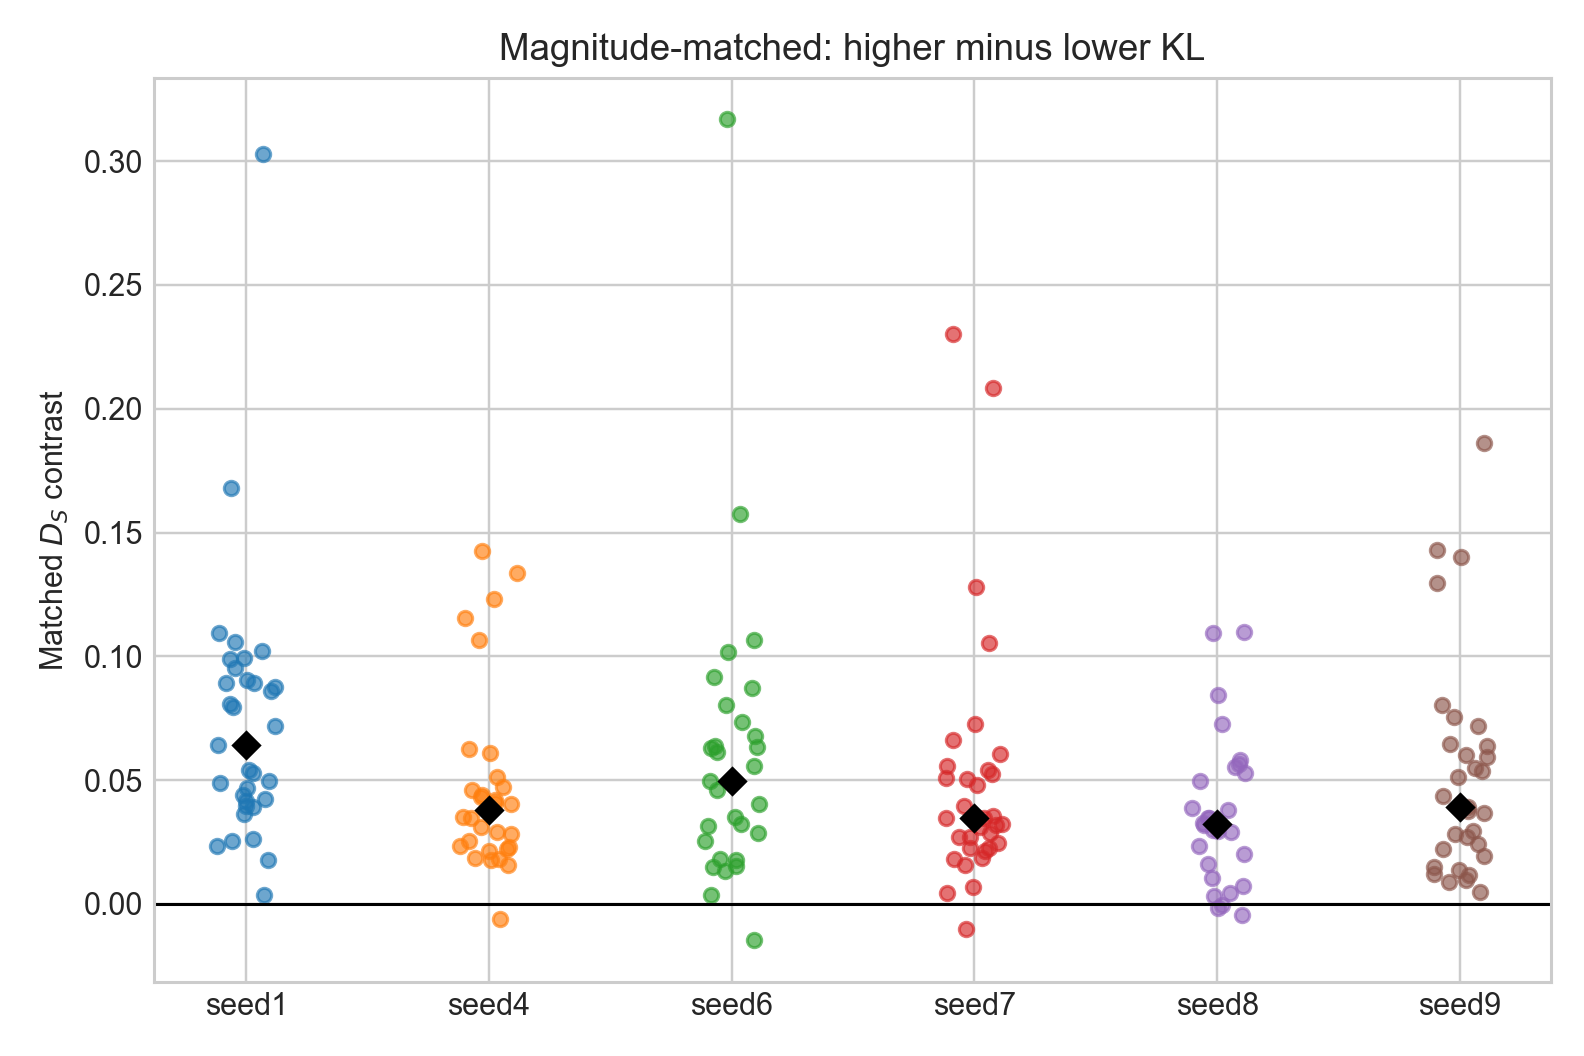
\includegraphics[width=\linewidth]{figures/draft2/fig2_magnitude_matched.png}
\\[-2mm]\small (a) Similar raw displacement, different functional damage
\end{minipage}\hfill
\begin{minipage}[t]{0.48\textwidth}\centering
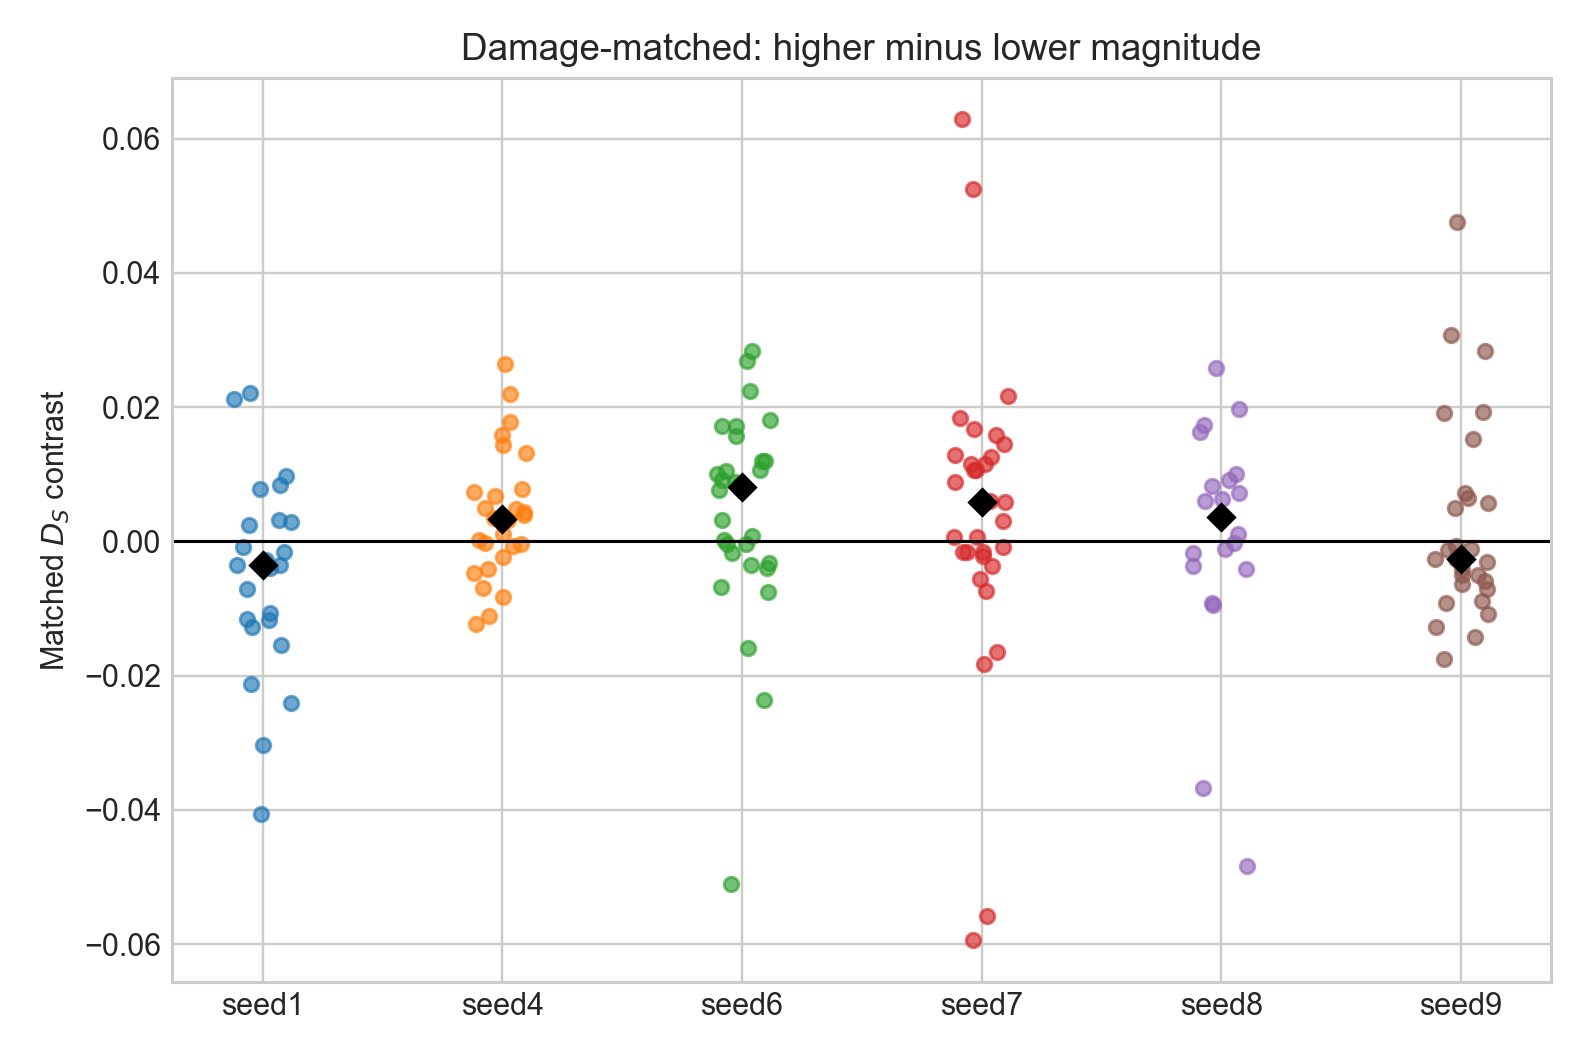
\includegraphics[width=\linewidth]{figures/draft2/fig2_damage_matched.png}
\\[-2mm]\small (b) Similar KL/NLL damage, different raw displacement
\end{minipage}
\caption{\textbf{Complementary matched contrasts within residual attenuation.}
Functional-damage differences retain a stable top-1 contrast at matched
magnitude, while the residual magnitude contrast is small after joint KL/NLL
matching. Points and intervals summarize independent runs, not tokens.}
\label{fig:damage}
\end{figure*}

Finally, KL, NLL, and $D_S$ are computed from the same intervened logits. The
matched design shows discrimination among measured descriptors; it does not
randomize KL/NLL or establish mediation.
